\documentclass[1p]{elsarticle_modified}
%\bibliographystyle{elsarticle-num}

%\usepackage[colorlinks]{hyperref}
%\usepackage{abbrmath_seonhwa} %\Abb, \Ascr, \Acal ,\Abf, \Afrak
\usepackage{amsfonts}
\usepackage{amssymb}
\usepackage{amsmath}
\usepackage{amsthm}
\usepackage{scalefnt}
\usepackage{amsbsy}
\usepackage{kotex}
\usepackage{caption}
\usepackage{subfig}
\usepackage{color}
\usepackage{graphicx}
\usepackage{xcolor} %% white, black, red, green, blue, cyan, magenta, yellow
\usepackage{float}
\usepackage{setspace}
\usepackage{hyperref}

\usepackage{tikz}
\usetikzlibrary{arrows}

\usepackage{multirow}
\usepackage{array} % fixed length table
\usepackage{hhline}

%%%%%%%%%%%%%%%%%%%%%
\makeatletter
\renewcommand*\env@matrix[1][\arraystretch]{%
	\edef\arraystretch{#1}%
	\hskip -\arraycolsep
	\let\@ifnextchar\new@ifnextchar
	\array{*\c@MaxMatrixCols c}}
\makeatother %https://tex.stackexchange.com/questions/14071/how-can-i-increase-the-line-spacing-in-a-matrix
%%%%%%%%%%%%%%%

\usepackage[normalem]{ulem}

\newcommand{\msout}[1]{\ifmmode\text{\sout{\ensuremath{#1}}}\else\sout{#1}\fi}
%SOURCE: \msout is \stkout macro in https://tex.stackexchange.com/questions/20609/strikeout-in-math-mode

\newcommand{\cancel}[1]{
	\ifmmode
	{\color{red}\msout{#1}}
	\else
	{\color{red}\sout{#1}}
	\fi
}

\newcommand{\add}[1]{
	{\color{blue}\uwave{#1}}
}

\newcommand{\replace}[2]{
	\ifmmode
	{\color{red}\msout{#1}}{\color{blue}\uwave{#2}}
	\else
	{\color{red}\sout{#1}}{\color{blue}\uwave{#2}}
	\fi
}

\newcommand{\Sol}{\mathcal{S}} %segment
\newcommand{\D}{D} %diagram
\newcommand{\A}{\mathcal{A}} %arc


%%%%%%%%%%%%%%%%%%%%%%%%%%%%%5 test

\def\sl{\operatorname{\textup{SL}}(2,\Cbb)}
\def\psl{\operatorname{\textup{PSL}}(2,\Cbb)}
\def\quan{\mkern 1mu \triangleright \mkern 1mu}

\theoremstyle{definition}
\newtheorem{thm}{Theorem}[section]
\newtheorem{prop}[thm]{Proposition}
\newtheorem{lem}[thm]{Lemma}
\newtheorem{ques}[thm]{Question}
\newtheorem{cor}[thm]{Corollary}
\newtheorem{defn}[thm]{Definition}
\newtheorem{exam}[thm]{Example}
\newtheorem{rmk}[thm]{Remark}
\newtheorem{alg}[thm]{Algorithm}

\newcommand{\I}{\sqrt{-1}}
\begin{document}

%\begin{frontmatter}
%
%\title{Boundary parabolic representations of knots up to 8 crossings}
%
%%% Group authors per affiliation:
%\author{Yunhi Cho} 
%\address{Department of Mathematics, University of Seoul, Seoul, Korea}
%\ead{yhcho@uos.ac.kr}
%
%
%\author{Seonhwa Kim} %\fnref{s_kim}}
%\address{Center for Geometry and Physics, Institute for Basic Science, Pohang, 37673, Korea}
%\ead{ryeona17@ibs.re.kr}
%
%\author{Hyuk Kim}
%\address{Department of Mathematical Sciences, Seoul National University, Seoul 08826, Korea}
%\ead{hyukkim@snu.ac.kr}
%
%\author{Seokbeom Yoon}
%\address{Department of Mathematical Sciences, Seoul National University, Seoul, 08826,  Korea}
%\ead{sbyoon15@snu.ac.kr}
%
%\begin{abstract}
%We find all boundary parabolic representation of knots up to 8 crossings.
%
%\end{abstract}
%\begin{keyword}
%    \MSC[2010] 57M25 
%\end{keyword}
%
%\end{frontmatter}

%\linenumbers
%\tableofcontents
%
\newcommand\colored[1]{\textcolor{white}{\rule[-0.35ex]{0.8em}{1.4ex}}\kern-0.8em\color{red} #1}%
%\newcommand\colored[1]{\textcolor{white}{ #1}\kern-2.17ex	\textcolor{white}{ #1}\kern-1.81ex	\textcolor{white}{ #1}\kern-2.15ex\color{red}#1	}

{\Large $\underline{11a_{171}~(K11a_{171})}$}

\setlength{\tabcolsep}{10pt}
\renewcommand{\arraystretch}{1.6}
\vspace{1cm}\begin{tabular}{m{100pt}>{\centering\arraybackslash}m{274pt}}
\multirow{5}{120pt}{
	\centering
	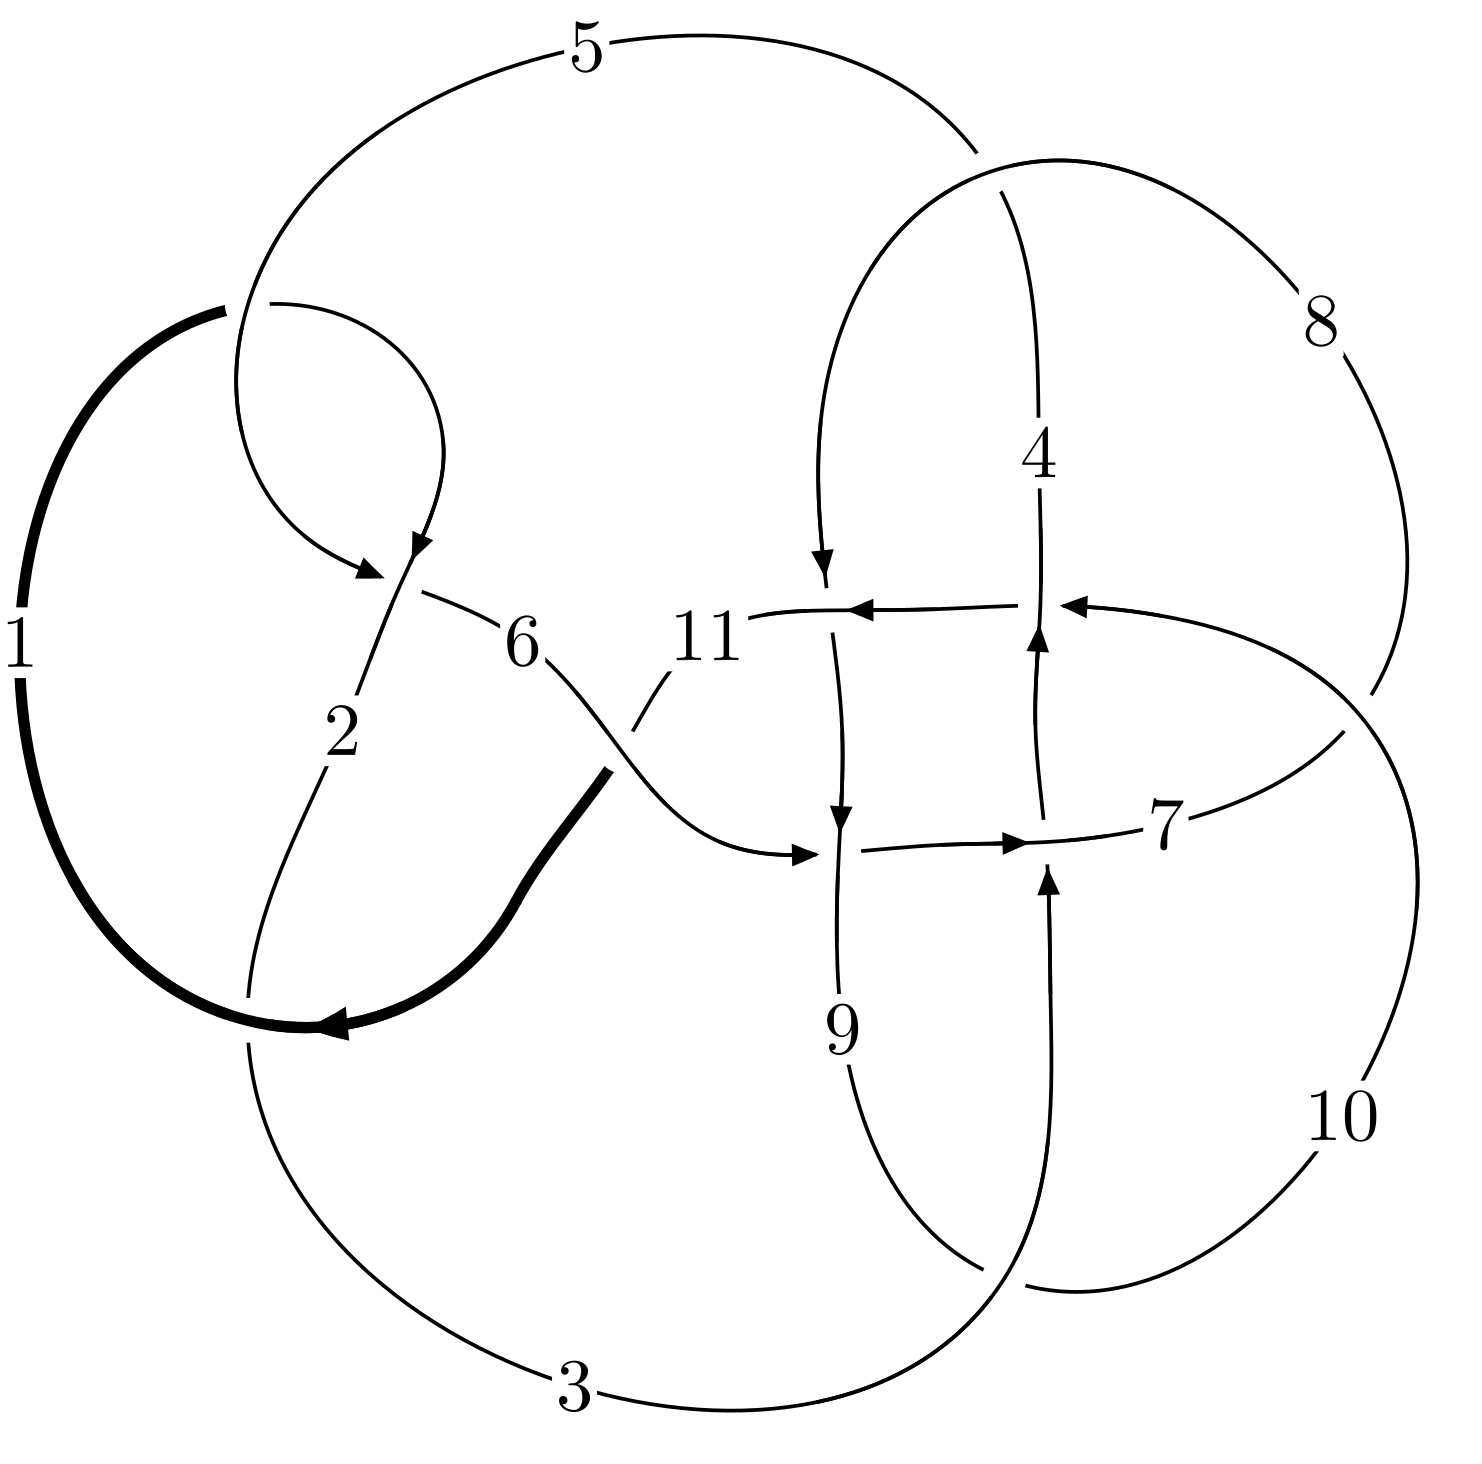
\includegraphics[width=112pt]{../../../GIT/diagram.site/Diagrams/png/420_11a_171.png}\\
\ \ \ A knot diagram\footnotemark}&
\allowdisplaybreaks
\textbf{Linearized knot diagam} \\
\cline{2-2}
 &
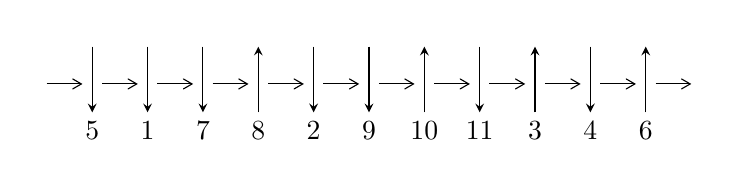
\begin{tikzpicture}[x=20pt, y=17pt]
	% nodes
	\node (C0) at (0, 0) {};
	\node (C1) at (1, 0) {};
	\node (C1U) at (1, +1) {};
	\node (C1D) at (1, -1) {5};

	\node (C2) at (2, 0) {};
	\node (C2U) at (2, +1) {};
	\node (C2D) at (2, -1) {1};

	\node (C3) at (3, 0) {};
	\node (C3U) at (3, +1) {};
	\node (C3D) at (3, -1) {7};

	\node (C4) at (4, 0) {};
	\node (C4U) at (4, +1) {};
	\node (C4D) at (4, -1) {8};

	\node (C5) at (5, 0) {};
	\node (C5U) at (5, +1) {};
	\node (C5D) at (5, -1) {2};

	\node (C6) at (6, 0) {};
	\node (C6U) at (6, +1) {};
	\node (C6D) at (6, -1) {9};

	\node (C7) at (7, 0) {};
	\node (C7U) at (7, +1) {};
	\node (C7D) at (7, -1) {10};

	\node (C8) at (8, 0) {};
	\node (C8U) at (8, +1) {};
	\node (C8D) at (8, -1) {11};

	\node (C9) at (9, 0) {};
	\node (C9U) at (9, +1) {};
	\node (C9D) at (9, -1) {3};

	\node (C10) at (10, 0) {};
	\node (C10U) at (10, +1) {};
	\node (C10D) at (10, -1) {4};

	\node (C11) at (11, 0) {};
	\node (C11U) at (11, +1) {};
	\node (C11D) at (11, -1) {6};
	\node (C12) at (12, 0) {};

	% arrows
	\draw[->,>={angle 60}]
	(C0) edge (C1) (C1) edge (C2) (C2) edge (C3) (C3) edge (C4) (C4) edge (C5) (C5) edge (C6) (C6) edge (C7) (C7) edge (C8) (C8) edge (C9) (C9) edge (C10) (C10) edge (C11) (C11) edge (C12) ;	\draw[->,>=stealth]
	(C1U) edge (C1D) (C2U) edge (C2D) (C3U) edge (C3D) (C4D) edge (C4U) (C5U) edge (C5D) (C6U) edge (C6D) (C7D) edge (C7U) (C8U) edge (C8D) (C9D) edge (C9U) (C10U) edge (C10D) (C11D) edge (C11U) ;
	\end{tikzpicture} \\
\hhline{~~} \\& 
\textbf{Solving Sequence} \\ \cline{2-2} 
 &
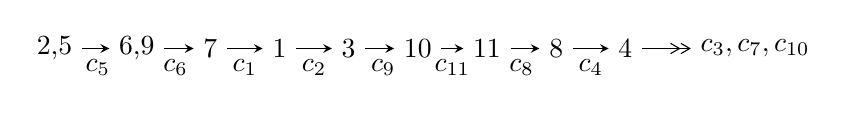
\begin{tikzpicture}[x=25pt, y=7pt]
	% node
	\node (A0) at (-1/8, 0) {2,5};
	\node (A1) at (17/16, 0) {6,9};
	\node (A2) at (17/8, 0) {7};
	\node (A3) at (25/8, 0) {1};
	\node (A4) at (33/8, 0) {3};
	\node (A5) at (41/8, 0) {10};
	\node (A6) at (49/8, 0) {11};
	\node (A7) at (57/8, 0) {8};
	\node (A8) at (65/8, 0) {4};
	\node (C1) at (1/2, -1) {$c_{5}$};
	\node (C2) at (13/8, -1) {$c_{6}$};
	\node (C3) at (21/8, -1) {$c_{1}$};
	\node (C4) at (29/8, -1) {$c_{2}$};
	\node (C5) at (37/8, -1) {$c_{9}$};
	\node (C6) at (45/8, -1) {$c_{11}$};
	\node (C7) at (53/8, -1) {$c_{8}$};
	\node (C8) at (61/8, -1) {$c_{4}$};
	\node (A9) at (10, 0) {$c_{3},c_{7},c_{10}$};

	% edge
	\draw[->,>=stealth]	
	(A0) edge (A1) (A1) edge (A2) (A2) edge (A3) (A3) edge (A4) (A4) edge (A5) (A5) edge (A6) (A6) edge (A7) (A7) edge (A8) ;
	\draw[->>,>={angle 60}]	
	(A8) edge (A9);
\end{tikzpicture} \\ 

\end{tabular} \\

\footnotetext{
The image of knot diagram is generated by the software ``\textbf{Draw programme}" developed by Andrew Bartholomew(\url{http://www.layer8.co.uk/maths/draw/index.htm\#Running-draw}), where we modified some parts for our purpose(\url{https://github.com/CATsTAILs/LinksPainter}).
}\phantom \\ \newline 
\centering \textbf{Ideals for irreducible components\footnotemark of $X_{\text{par}}$} 
 
\begin{align*}
I^u_{1}&=\langle 
519990 u^{45}+1958497 u^{44}+\cdots+69383 b+409894,\\
\phantom{I^u_{1}}&\phantom{= \langle  }430369 u^{45}+1395316 u^{44}+\cdots+69383 a+63169,\;u^{46}+5 u^{45}+\cdots+5 u+1\rangle \\
I^u_{2}&=\langle 
-29 u^{30} a+623 u^{30}+\cdots+2 a-1427,\;2 u^{29} a-2 u^{30}+\cdots+2 a+2,\;u^{31}-2 u^{30}+\cdots-2 u+1\rangle \\
I^u_{3}&=\langle 
2 u^{14}- u^{13}-7 u^{12}+6 u^{11}+12 u^{10}-13 u^9-10 u^8+15 u^7+4 u^6-9 u^5+2 u^4+2 u^3-3 u^2+b- u+2,\\
\phantom{I^u_{3}}&\phantom{= \langle  }- u^{15}+3 u^{14}+\cdots+a+3,\\
\phantom{I^u_{3}}&\phantom{= \langle  }u^{16}-2 u^{15}-2 u^{14}+8 u^{13}- u^{12}-14 u^{11}+10 u^{10}+11 u^9-15 u^8- u^7+11 u^6-6 u^5-2 u^4+4 u^3-2 u+1\rangle \\
I^u_{4}&=\langle 
b- a-1,\;a^2+3 a+1,\;u+1\rangle \\
\\
I^v_{1}&=\langle 
a,\;b-1,\;v-1\rangle \\
\end{align*}
\raggedright * 5 irreducible components of $\dim_{\mathbb{C}}=0$, with total 127 representations.\\
\footnotetext{All coefficients of polynomials are rational numbers. But the coefficients are sometimes approximated in decimal forms when there is not enough margin.}
\newpage
\renewcommand{\arraystretch}{1}
\centering \section*{I. $I^u_{1}= \langle 5.20\times10^{5} u^{45}+1.96\times10^{6} u^{44}+\cdots+6.94\times10^{4} b+4.10\times10^{5},\;4.30\times10^{5} u^{45}+1.40\times10^{6} u^{44}+\cdots+6.94\times10^{4} a+6.32\times10^{4},\;u^{46}+5 u^{45}+\cdots+5 u+1 \rangle$}
\flushleft \textbf{(i) Arc colorings}\\
\begin{tabular}{m{7pt} m{180pt} m{7pt} m{180pt} }
\flushright $a_{2}=$&$\begin{pmatrix}0\\u\end{pmatrix}$ \\
\flushright $a_{5}=$&$\begin{pmatrix}1\\0\end{pmatrix}$ \\
\flushright $a_{6}=$&$\begin{pmatrix}1\\u^2\end{pmatrix}$ \\
\flushright $a_{9}=$&$\begin{pmatrix}-6.20280 u^{45}-20.1103 u^{44}+\cdots-3.24905 u-0.910439\\-7.49449 u^{45}-28.2273 u^{44}+\cdots-26.5100 u-5.90770\end{pmatrix}$ \\
\flushright $a_{7}=$&$\begin{pmatrix}-8.99833 u^{45}-31.6872 u^{44}+\cdots-10.4069 u-1.60077\\-5.46625 u^{45}-23.1524 u^{44}+\cdots-24.6669 u-5.54479\end{pmatrix}$ \\
\flushright $a_{1}=$&$\begin{pmatrix}u\\u\end{pmatrix}$ \\
\flushright $a_{3}=$&$\begin{pmatrix}- u^3\\- u^3+u\end{pmatrix}$ \\
\flushright $a_{10}=$&$\begin{pmatrix}-6.82680 u^{45}-25.1173 u^{44}+\cdots-11.4935 u-3.08978\\-5.46625 u^{45}-22.1524 u^{44}+\cdots-23.6669 u-5.54479\end{pmatrix}$ \\
\flushright $a_{11}=$&$\begin{pmatrix}u^3\\u^5- u^3+u\end{pmatrix}$ \\
\flushright $a_{8}=$&$\begin{pmatrix}-4.24914 u^{45}-18.3303 u^{44}+\cdots-13.4790 u-4.32022\\-2.54225 u^{45}-10.0590 u^{44}+\cdots-8.86675 u-1.62373\end{pmatrix}$ \\
\flushright $a_{4}=$&$\begin{pmatrix}-6.16768 u^{45}-23.6777 u^{44}+\cdots-9.23804 u-2.10931\\-6.74815 u^{45}-29.0939 u^{44}+\cdots-27.8357 u-6.23964\end{pmatrix}$\\ \flushright $a_{4}=$&$\begin{pmatrix}-6.16768 u^{45}-23.6777 u^{44}+\cdots-9.23804 u-2.10931\\-6.74815 u^{45}-29.0939 u^{44}+\cdots-27.8357 u-6.23964\end{pmatrix}$\\&\end{tabular}
\flushleft \textbf{(ii) Obstruction class $= -1$}\\~\\
\flushleft \textbf{(iii) Cusp Shapes $= -\frac{130759}{69383} u^{45}+\frac{81491}{69383} u^{44}+\cdots-\frac{583416}{69383} u-\frac{777173}{69383}$}\\~\\
\newpage\renewcommand{\arraystretch}{1}
\flushleft \textbf{(iv) u-Polynomials at the component}\newline \\
\begin{tabular}{m{50pt}|m{274pt}}
Crossings & \hspace{64pt}u-Polynomials at each crossing \\
\hline $$\begin{aligned}c_{1},c_{5}\end{aligned}$$&$\begin{aligned}
&u^{46}+5 u^{45}+\cdots+5 u+1
\end{aligned}$\\
\hline $$\begin{aligned}c_{2}\end{aligned}$$&$\begin{aligned}
&u^{46}+23 u^{45}+\cdots-11 u+1
\end{aligned}$\\
\hline $$\begin{aligned}c_{3},c_{10}\end{aligned}$$&$\begin{aligned}
&u^{46}- u^{45}+\cdots+2 u+1
\end{aligned}$\\
\hline $$\begin{aligned}c_{4},c_{9}\end{aligned}$$&$\begin{aligned}
&u^{46}-2 u^{45}+\cdots+u+1
\end{aligned}$\\
\hline $$\begin{aligned}c_{6},c_{8}\end{aligned}$$&$\begin{aligned}
&u^{46}+6 u^{45}+\cdots-9 u+1
\end{aligned}$\\
\hline $$\begin{aligned}c_{7}\end{aligned}$$&$\begin{aligned}
&u^{46}+26 u^{45}+\cdots+u+1
\end{aligned}$\\
\hline $$\begin{aligned}c_{11}\end{aligned}$$&$\begin{aligned}
&u^{46}+15 u^{45}+\cdots+1885 u+149
\end{aligned}$\\
\hline
\end{tabular}\\~\\
\newpage\renewcommand{\arraystretch}{1}
\flushleft \textbf{(v) Riley Polynomials at the component}\newline \\
\begin{tabular}{m{50pt}|m{274pt}}
Crossings & \hspace{64pt}Riley Polynomials at each crossing \\
\hline $$\begin{aligned}c_{1},c_{5}\end{aligned}$$&$\begin{aligned}
&y^{46}-23 y^{45}+\cdots+11 y+1
\end{aligned}$\\
\hline $$\begin{aligned}c_{2}\end{aligned}$$&$\begin{aligned}
&y^{46}+5 y^{45}+\cdots-73 y+1
\end{aligned}$\\
\hline $$\begin{aligned}c_{3},c_{10}\end{aligned}$$&$\begin{aligned}
&y^{46}-19 y^{45}+\cdots-52 y+1
\end{aligned}$\\
\hline $$\begin{aligned}c_{4},c_{9}\end{aligned}$$&$\begin{aligned}
&y^{46}-2 y^{45}+\cdots+27 y+1
\end{aligned}$\\
\hline $$\begin{aligned}c_{6},c_{8}\end{aligned}$$&$\begin{aligned}
&y^{46}-30 y^{45}+\cdots-121 y+1
\end{aligned}$\\
\hline $$\begin{aligned}c_{7}\end{aligned}$$&$\begin{aligned}
&y^{46}+38 y^{44}+\cdots+49 y+1
\end{aligned}$\\
\hline $$\begin{aligned}c_{11}\end{aligned}$$&$\begin{aligned}
&y^{46}+13 y^{45}+\cdots+238229 y+22201
\end{aligned}$\\
\hline
\end{tabular}\\~\\
\newpage\flushleft \textbf{(vi) Complex Volumes and Cusp Shapes}
$$\begin{array}{c|c|c}  
\text{Solutions to }I^u_{1}& \I (\text{vol} + \sqrt{-1}CS) & \text{Cusp shape}\\
 \hline 
\begin{aligned}
u &= -0.933486 + 0.444661 I \\
a &= \phantom{-}1.39390 - 0.39376 I \\
b &= \phantom{-}0.917537 - 0.675621 I\end{aligned}
 & -1.098380 + 0.644192 I & -5.70718 - 0.44366 I \\ \hline\begin{aligned}
u &= -0.933486 - 0.444661 I \\
a &= \phantom{-}1.39390 + 0.39376 I \\
b &= \phantom{-}0.917537 + 0.675621 I\end{aligned}
 & -1.098380 - 0.644192 I & -5.70718 + 0.44366 I \\ \hline\begin{aligned}
u &= -0.751399 + 0.721194 I \\
a &= \phantom{-}0.377914 + 0.652284 I \\
b &= -0.232701 + 0.476942 I\end{aligned}
 & \phantom{-}1.87378 + 10.77040 I & -1.30875 - 9.40079 I \\ \hline\begin{aligned}
u &= -0.751399 - 0.721194 I \\
a &= \phantom{-}0.377914 - 0.652284 I \\
b &= -0.232701 - 0.476942 I\end{aligned}
 & \phantom{-}1.87378 - 10.77040 I & -1.30875 + 9.40079 I \\ \hline\begin{aligned}
u &= -0.856947 + 0.701617 I \\
a &= -0.552390 + 0.650998 I \\
b &= -0.148213 + 0.105841 I\end{aligned}
 & \phantom{-}1.57181 - 5.40355 I & -1.95277 + 5.01520 I \\ \hline\begin{aligned}
u &= -0.856947 - 0.701617 I \\
a &= -0.552390 - 0.650998 I \\
b &= -0.148213 - 0.105841 I\end{aligned}
 & \phantom{-}1.57181 + 5.40355 I & -1.95277 - 5.01520 I \\ \hline\begin{aligned}
u &= -0.291347 + 0.840599 I \\
a &= \phantom{-}0.415288 - 0.440575 I \\
b &= -1.79617 - 0.89753 I\end{aligned}
 & -0.71987 - 13.43220 I & -2.36696 + 7.45298 I \\ \hline\begin{aligned}
u &= -0.291347 - 0.840599 I \\
a &= \phantom{-}0.415288 + 0.440575 I \\
b &= -1.79617 + 0.89753 I\end{aligned}
 & -0.71987 + 13.43220 I & -2.36696 - 7.45298 I \\ \hline\begin{aligned}
u &= -0.132938 + 0.848595 I \\
a &= \phantom{-}0.159620 - 0.433157 I \\
b &= -0.956107 + 0.290168 I\end{aligned}
 & -2.72587 + 3.54069 I & -7.48667 - 4.84167 I \\ \hline\begin{aligned}
u &= -0.132938 - 0.848595 I \\
a &= \phantom{-}0.159620 + 0.433157 I \\
b &= -0.956107 - 0.290168 I\end{aligned}
 & -2.72587 - 3.54069 I & -7.48667 + 4.84167 I\\
 \hline 
 \end{array}$$\newpage$$\begin{array}{c|c|c}  
\text{Solutions to }I^u_{1}& \I (\text{vol} + \sqrt{-1}CS) & \text{Cusp shape}\\
 \hline 
\begin{aligned}
u &= -0.660174 + 0.548978 I \\
a &= \phantom{-}0.018944 - 1.119640 I \\
b &= -0.023291 - 1.106980 I\end{aligned}
 & -0.36479 + 3.45703 I & -5.70781 - 7.10352 I \\ \hline\begin{aligned}
u &= -0.660174 - 0.548978 I \\
a &= \phantom{-}0.018944 + 1.119640 I \\
b &= -0.023291 + 1.106980 I\end{aligned}
 & -0.36479 - 3.45703 I & -5.70781 + 7.10352 I \\ \hline\begin{aligned}
u &= \phantom{-}1.112300 + 0.261314 I \\
a &= -1.89980 - 0.01447 I \\
b &= -0.856736 - 0.971479 I\end{aligned}
 & -5.91551 - 1.58146 I & -13.59206 + 3.66934 I \\ \hline\begin{aligned}
u &= \phantom{-}1.112300 - 0.261314 I \\
a &= -1.89980 + 0.01447 I \\
b &= -0.856736 + 0.971479 I\end{aligned}
 & -5.91551 + 1.58146 I & -13.59206 - 3.66934 I \\ \hline\begin{aligned}
u &= \phantom{-}1.135200 + 0.294115 I \\
a &= -1.85511 + 1.41022 I \\
b &= -1.71754 - 0.41559 I\end{aligned}
 & -6.20814 + 1.80497 I & -14.2464 - 4.3963 I \\ \hline\begin{aligned}
u &= \phantom{-}1.135200 - 0.294115 I \\
a &= -1.85511 - 1.41022 I \\
b &= -1.71754 + 0.41559 I\end{aligned}
 & -6.20814 - 1.80497 I & -14.2464 + 4.3963 I \\ \hline\begin{aligned}
u &= -0.375652 + 0.726957 I \\
a &= \phantom{-}0.249990 + 0.342484 I \\
b &= \phantom{-}1.203890 - 0.206841 I\end{aligned}
 & -1.60276 - 0.98411 I & -7.53408 + 0.28472 I \\ \hline\begin{aligned}
u &= -0.375652 - 0.726957 I \\
a &= \phantom{-}0.249990 - 0.342484 I \\
b &= \phantom{-}1.203890 + 0.206841 I\end{aligned}
 & -1.60276 + 0.98411 I & -7.53408 - 0.28472 I \\ \hline\begin{aligned}
u &= \phantom{-}0.881986 + 0.787307 I \\
a &= \phantom{-}0.191650 - 0.055578 I \\
b &= -0.053824 + 0.253337 I\end{aligned}
 & \phantom{-}3.98279 - 2.95487 I & \phantom{-}23.7349 - 13.5735 I \\ \hline\begin{aligned}
u &= \phantom{-}0.881986 - 0.787307 I \\
a &= \phantom{-}0.191650 + 0.055578 I \\
b &= -0.053824 - 0.253337 I\end{aligned}
 & \phantom{-}3.98279 + 2.95487 I & \phantom{-}23.7349 + 13.5735 I\\
 \hline 
 \end{array}$$\newpage$$\begin{array}{c|c|c}  
\text{Solutions to }I^u_{1}& \I (\text{vol} + \sqrt{-1}CS) & \text{Cusp shape}\\
 \hline 
\begin{aligned}
u &= -1.099790 + 0.438913 I \\
a &= -1.83196 - 1.36948 I \\
b &= -2.21067 - 0.24014 I\end{aligned}
 & -4.28647 + 3.53114 I & -10.17349 - 4.71484 I \\ \hline\begin{aligned}
u &= -1.099790 - 0.438913 I \\
a &= -1.83196 + 1.36948 I \\
b &= -2.21067 + 0.24014 I\end{aligned}
 & -4.28647 - 3.53114 I & -10.17349 + 4.71484 I \\ \hline\begin{aligned}
u &= \phantom{-}1.059210 + 0.534264 I \\
a &= \phantom{-}0.541434 - 0.766541 I \\
b &= \phantom{-}0.805091 + 0.458424 I\end{aligned}
 & \phantom{-}0.17597 - 5.33365 I & -1.16724 + 4.83689 I \\ \hline\begin{aligned}
u &= \phantom{-}1.059210 - 0.534264 I \\
a &= \phantom{-}0.541434 + 0.766541 I \\
b &= \phantom{-}0.805091 - 0.458424 I\end{aligned}
 & \phantom{-}0.17597 + 5.33365 I & -1.16724 - 4.83689 I \\ \hline\begin{aligned}
u &= \phantom{-}1.099340 + 0.465407 I \\
a &= -1.63134 + 0.89715 I \\
b &= -1.21983 - 1.23467 I\end{aligned}
 & -4.10186 - 3.81474 I & -9.79702 + 3.58298 I \\ \hline\begin{aligned}
u &= \phantom{-}1.099340 - 0.465407 I \\
a &= -1.63134 - 0.89715 I \\
b &= -1.21983 + 1.23467 I\end{aligned}
 & -4.10186 + 3.81474 I & -9.79702 - 3.58298 I \\ \hline\begin{aligned}
u &= -0.278150 + 0.732712 I \\
a &= -0.376095 + 0.785335 I \\
b &= \phantom{-}1.76661 + 0.88827 I\end{aligned}
 & -2.03242 - 4.83583 I & -8.60020 + 6.83106 I \\ \hline\begin{aligned}
u &= -0.278150 - 0.732712 I \\
a &= -0.376095 - 0.785335 I \\
b &= \phantom{-}1.76661 - 0.88827 I\end{aligned}
 & -2.03242 + 4.83583 I & -8.60020 - 6.83106 I \\ \hline\begin{aligned}
u &= -0.761418 + 0.115983 I \\
a &= \phantom{-}0.858924 - 0.607457 I \\
b &= \phantom{-}0.637850 - 0.558762 I\end{aligned}
 & -1.37145 + 0.34774 I & -7.35312 - 1.68014 I \\ \hline\begin{aligned}
u &= -0.761418 - 0.115983 I \\
a &= \phantom{-}0.858924 + 0.607457 I \\
b &= \phantom{-}0.637850 + 0.558762 I\end{aligned}
 & -1.37145 - 0.34774 I & -7.35312 + 1.68014 I\\
 \hline 
 \end{array}$$\newpage$$\begin{array}{c|c|c}  
\text{Solutions to }I^u_{1}& \I (\text{vol} + \sqrt{-1}CS) & \text{Cusp shape}\\
 \hline 
\begin{aligned}
u &= \phantom{-}1.215530 + 0.243371 I \\
a &= \phantom{-}1.75500 - 1.20403 I \\
b &= \phantom{-}1.83289 + 0.11458 I\end{aligned}
 & -5.60396 + 10.10350 I & -8.00817 - 5.63549 I \\ \hline\begin{aligned}
u &= \phantom{-}1.215530 - 0.243371 I \\
a &= \phantom{-}1.75500 + 1.20403 I \\
b &= \phantom{-}1.83289 - 0.11458 I\end{aligned}
 & -5.60396 - 10.10350 I & -8.00817 + 5.63549 I \\ \hline\begin{aligned}
u &= \phantom{-}0.431319 + 0.618019 I \\
a &= \phantom{-}0.744120 - 0.125502 I \\
b &= -0.551257 + 0.192009 I\end{aligned}
 & \phantom{-}2.00312 + 0.77598 I & \phantom{-}3.08048 - 0.37837 I \\ \hline\begin{aligned}
u &= \phantom{-}0.431319 - 0.618019 I \\
a &= \phantom{-}0.744120 + 0.125502 I \\
b &= -0.551257 - 0.192009 I\end{aligned}
 & \phantom{-}2.00312 - 0.77598 I & \phantom{-}3.08048 + 0.37837 I \\ \hline\begin{aligned}
u &= -1.115390 + 0.573899 I \\
a &= -1.01263 - 1.47969 I \\
b &= -1.60084 - 0.24549 I\end{aligned}
 & -3.77845 + 5.97580 I & -9.62613 - 4.25022 I \\ \hline\begin{aligned}
u &= -1.115390 - 0.573899 I \\
a &= -1.01263 + 1.47969 I \\
b &= -1.60084 + 0.24549 I\end{aligned}
 & -3.77845 - 5.97580 I & -9.62613 + 4.25022 I \\ \hline\begin{aligned}
u &= -1.133410 + 0.543345 I \\
a &= -2.66832 - 1.09843 I \\
b &= -2.59106 + 0.99651 I\end{aligned}
 & -4.51494 + 9.66961 I & -12.1786 - 10.5958 I \\ \hline\begin{aligned}
u &= -1.133410 - 0.543345 I \\
a &= -2.66832 + 1.09843 I \\
b &= -2.59106 - 0.99651 I\end{aligned}
 & -4.51494 - 9.66961 I & -12.1786 + 10.5958 I \\ \hline\begin{aligned}
u &= \phantom{-}1.225340 + 0.349011 I \\
a &= \phantom{-}1.355770 - 0.047043 I \\
b &= \phantom{-}0.889349 + 1.016990 I\end{aligned}
 & -6.99619 - 7.57481 I & -10.39877 + 7.23305 I \\ \hline\begin{aligned}
u &= \phantom{-}1.225340 - 0.349011 I \\
a &= \phantom{-}1.355770 + 0.047043 I \\
b &= \phantom{-}0.889349 - 1.016990 I\end{aligned}
 & -6.99619 + 7.57481 I & -10.39877 - 7.23305 I\\
 \hline 
 \end{array}$$\newpage$$\begin{array}{c|c|c}  
\text{Solutions to }I^u_{1}& \I (\text{vol} + \sqrt{-1}CS) & \text{Cusp shape}\\
 \hline 
\begin{aligned}
u &= -1.197320 + 0.502148 I \\
a &= \phantom{-}1.031320 + 0.860349 I \\
b &= \phantom{-}1.50432 - 0.00862 I\end{aligned}
 & -5.94279 + 1.33870 I & \phantom{-0.000000 } 0 \\ \hline\begin{aligned}
u &= -1.197320 - 0.502148 I \\
a &= \phantom{-}1.031320 - 0.860349 I \\
b &= \phantom{-}1.50432 + 0.00862 I\end{aligned}
 & -5.94279 - 1.33870 I & \phantom{-0.000000 } 0 \\ \hline\begin{aligned}
u &= -1.165270 + 0.576600 I \\
a &= \phantom{-}2.37516 + 1.00046 I \\
b &= \phantom{-}2.36478 - 1.14677 I\end{aligned}
 & -3.3293 + 18.6712 I & \phantom{-0.000000 } 0 \\ \hline\begin{aligned}
u &= -1.165270 - 0.576600 I \\
a &= \phantom{-}2.37516 - 1.00046 I \\
b &= \phantom{-}2.36478 + 1.14677 I\end{aligned}
 & -3.3293 - 18.6712 I & \phantom{-0.000000 } 0 \\ \hline\begin{aligned}
u &= \phantom{-}0.092447 + 0.293184 I \\
a &= -1.64140 + 2.88752 I \\
b &= \phantom{-}1.035920 - 0.158140 I\end{aligned}
 & -1.65225 + 0.00944 I & -6.31613 + 0.26061 I \\ \hline\begin{aligned}
u &= \phantom{-}0.092447 - 0.293184 I \\
a &= -1.64140 - 2.88752 I \\
b &= \phantom{-}1.035920 + 0.158140 I\end{aligned}
 & -1.65225 - 0.00944 I & -6.31613 - 0.26061 I\\
 \hline 
 \end{array}$$\newpage\newpage\renewcommand{\arraystretch}{1}
\centering \section*{II. $I^u_{2}= \langle -29 u^{30} a+623 u^{30}+\cdots+2 a-1427,\;2 u^{29} a-2 u^{30}+\cdots+2 a+2,\;u^{31}-2 u^{30}+\cdots-2 u+1 \rangle$}
\flushleft \textbf{(i) Arc colorings}\\
\begin{tabular}{m{7pt} m{180pt} m{7pt} m{180pt} }
\flushright $a_{2}=$&$\begin{pmatrix}0\\u\end{pmatrix}$ \\
\flushright $a_{5}=$&$\begin{pmatrix}1\\0\end{pmatrix}$ \\
\flushright $a_{6}=$&$\begin{pmatrix}1\\u^2\end{pmatrix}$ \\
\flushright $a_{9}=$&$\begin{pmatrix}a\\0.0368488 a u^{30}-0.791614 u^{30}+\cdots-0.00254130 a+1.81321\end{pmatrix}$ \\
\flushright $a_{7}=$&$\begin{pmatrix}1.79161 a u^{30}-1.31639 u^{30}+\cdots-0.813215 a+1.22872\\0.416773 a u^{30}+2.63278 u^{30}+\cdots-0.373571 a-3.45743\end{pmatrix}$ \\
\flushright $a_{1}=$&$\begin{pmatrix}u\\u\end{pmatrix}$ \\
\flushright $a_{3}=$&$\begin{pmatrix}- u^3\\- u^3+u\end{pmatrix}$ \\
\flushright $a_{10}=$&$\begin{pmatrix}0.0368488 a u^{30}+2.20839 u^{30}+\cdots+0.997459 a-2.18679\\0.108005 a u^{30}-0.561626 u^{30}+\cdots-0.0419314 a+1.41804\end{pmatrix}$ \\
\flushright $a_{11}=$&$\begin{pmatrix}u^3\\u^5- u^3+u\end{pmatrix}$ \\
\flushright $a_{8}=$&$\begin{pmatrix}0.0368488 a u^{30}+2.20839 u^{30}+\cdots+0.997459 a-2.18679\\-0.0368488 a u^{30}+0.791614 u^{30}+\cdots+0.00254130 a+0.186785\end{pmatrix}$ \\
\flushright $a_{4}=$&$\begin{pmatrix}-1.14485 a u^{30}+0.353240 u^{30}+\cdots+0.0444727 a-0.231258\\-0.0635324 a u^{30}+2.33037 u^{30}+\cdots+0.142313 a-3.54003\end{pmatrix}$\\ \flushright $a_{4}=$&$\begin{pmatrix}-1.14485 a u^{30}+0.353240 u^{30}+\cdots+0.0444727 a-0.231258\\-0.0635324 a u^{30}+2.33037 u^{30}+\cdots+0.142313 a-3.54003\end{pmatrix}$\\&\end{tabular}
\flushleft \textbf{(ii) Obstruction class $= -1$}\\~\\
\flushleft \textbf{(iii) Cusp Shapes $= 11 u^{30}-17 u^{29}-77 u^{28}+156 u^{27}+228 u^{26}-647 u^{25}-267 u^{24}+1574 u^{23}-282 u^{22}-2362 u^{21}+1582 u^{20}+2004 u^{19}-2748 u^{18}-365 u^{17}+2591 u^{16}-1168 u^{15}-1234 u^{14}+1358 u^{13}+106 u^{12}-640 u^{11}+136 u^{10}+174 u^9-30 u^8-92 u^7+60 u^6+44 u^5-44 u^4+16 u^3+11 u-11$}\\~\\
\newpage\renewcommand{\arraystretch}{1}
\flushleft \textbf{(iv) u-Polynomials at the component}\newline \\
\begin{tabular}{m{50pt}|m{274pt}}
Crossings & \hspace{64pt}u-Polynomials at each crossing \\
\hline $$\begin{aligned}c_{1},c_{5}\end{aligned}$$&$\begin{aligned}
&(u^{31}-2 u^{30}+\cdots-2 u+1)^{2}
\end{aligned}$\\
\hline $$\begin{aligned}c_{2}\end{aligned}$$&$\begin{aligned}
&(u^{31}+16 u^{30}+\cdots+2 u+1)^{2}
\end{aligned}$\\
\hline $$\begin{aligned}c_{3},c_{10}\end{aligned}$$&$\begin{aligned}
&u^{62}+2 u^{61}+\cdots+u-1
\end{aligned}$\\
\hline $$\begin{aligned}c_{4},c_{9}\end{aligned}$$&$\begin{aligned}
&u^{62}+2 u^{61}+\cdots-211 u+31
\end{aligned}$\\
\hline $$\begin{aligned}c_{6},c_{8}\end{aligned}$$&$\begin{aligned}
&u^{62}-3 u^{61}+\cdots+378 u-49
\end{aligned}$\\
\hline $$\begin{aligned}c_{7}\end{aligned}$$&$\begin{aligned}
&(u^{31}-15 u^{30}+\cdots+3 u-2)^{2}
\end{aligned}$\\
\hline $$\begin{aligned}c_{11}\end{aligned}$$&$\begin{aligned}
&(u^{31}-9 u^{30}+\cdots+73 u-8)^{2}
\end{aligned}$\\
\hline
\end{tabular}\\~\\
\newpage\renewcommand{\arraystretch}{1}
\flushleft \textbf{(v) Riley Polynomials at the component}\newline \\
\begin{tabular}{m{50pt}|m{274pt}}
Crossings & \hspace{64pt}Riley Polynomials at each crossing \\
\hline $$\begin{aligned}c_{1},c_{5}\end{aligned}$$&$\begin{aligned}
&(y^{31}-16 y^{30}+\cdots+2 y-1)^{2}
\end{aligned}$\\
\hline $$\begin{aligned}c_{2}\end{aligned}$$&$\begin{aligned}
&(y^{31}+28 y^{29}+\cdots-14 y-1)^{2}
\end{aligned}$\\
\hline $$\begin{aligned}c_{3},c_{10}\end{aligned}$$&$\begin{aligned}
&y^{62}+12 y^{61}+\cdots+29 y+1
\end{aligned}$\\
\hline $$\begin{aligned}c_{4},c_{9}\end{aligned}$$&$\begin{aligned}
&y^{62}+58 y^{60}+\cdots-104599 y+961
\end{aligned}$\\
\hline $$\begin{aligned}c_{6},c_{8}\end{aligned}$$&$\begin{aligned}
&y^{62}+13 y^{61}+\cdots+17738 y+2401
\end{aligned}$\\
\hline $$\begin{aligned}c_{7}\end{aligned}$$&$\begin{aligned}
&(y^{31}-3 y^{30}+\cdots+69 y-4)^{2}
\end{aligned}$\\
\hline $$\begin{aligned}c_{11}\end{aligned}$$&$\begin{aligned}
&(y^{31}+13 y^{30}+\cdots+833 y-64)^{2}
\end{aligned}$\\
\hline
\end{tabular}\\~\\
\newpage\flushleft \textbf{(vi) Complex Volumes and Cusp Shapes}
$$\begin{array}{c|c|c}  
\text{Solutions to }I^u_{2}& \I (\text{vol} + \sqrt{-1}CS) & \text{Cusp shape}\\
 \hline 
\begin{aligned}
u &= \phantom{-}0.790665 + 0.695036 I \\
a &= \phantom{-}0.669170 - 0.332267 I \\
b &= \phantom{-}0.0656518 + 0.0523021 I\end{aligned}
 & \phantom{-}3.79486 - 2.62922 I & \phantom{-}6.53544 + 4.19495 I \\ \hline\begin{aligned}
u &= \phantom{-}0.790665 + 0.695036 I \\
a &= -0.207742 + 0.086773 I \\
b &= -0.126798 + 0.478191 I\end{aligned}
 & \phantom{-}3.79486 - 2.62922 I & \phantom{-}6.53544 + 4.19495 I \\ \hline\begin{aligned}
u &= \phantom{-}0.790665 - 0.695036 I \\
a &= \phantom{-}0.669170 + 0.332267 I \\
b &= \phantom{-}0.0656518 - 0.0523021 I\end{aligned}
 & \phantom{-}3.79486 + 2.62922 I & \phantom{-}6.53544 - 4.19495 I \\ \hline\begin{aligned}
u &= \phantom{-}0.790665 - 0.695036 I \\
a &= -0.207742 - 0.086773 I \\
b &= -0.126798 - 0.478191 I\end{aligned}
 & \phantom{-}3.79486 + 2.62922 I & \phantom{-}6.53544 - 4.19495 I \\ \hline\begin{aligned}
u &= \phantom{-}0.271790 + 0.844936 I \\
a &= \phantom{-}0.569593 + 0.287323 I \\
b &= -1.48334 + 0.65965 I\end{aligned}
 & \phantom{-}0.86287 + 5.06730 I & \phantom{-}2.75638 - 8.05298 I \\ \hline\begin{aligned}
u &= \phantom{-}0.271790 + 0.844936 I \\
a &= -0.119874 - 0.268542 I \\
b &= \phantom{-}0.884101 - 0.757543 I\end{aligned}
 & \phantom{-}0.86287 + 5.06730 I & \phantom{-}2.75638 - 8.05298 I \\ \hline\begin{aligned}
u &= \phantom{-}0.271790 - 0.844936 I \\
a &= \phantom{-}0.569593 - 0.287323 I \\
b &= -1.48334 - 0.65965 I\end{aligned}
 & \phantom{-}0.86287 - 5.06730 I & \phantom{-}2.75638 + 8.05298 I \\ \hline\begin{aligned}
u &= \phantom{-}0.271790 - 0.844936 I \\
a &= -0.119874 + 0.268542 I \\
b &= \phantom{-}0.884101 + 0.757543 I\end{aligned}
 & \phantom{-}0.86287 - 5.06730 I & \phantom{-}2.75638 + 8.05298 I \\ \hline\begin{aligned}
u &= -1.11799\phantom{ +0.000000I} \\
a &= -0.284257\phantom{ +0.000000I} \\
b &= \phantom{-}0.391788\phantom{ +0.000000I}\end{aligned}
 & -2.94773\phantom{ +0.000000I} & \phantom{-}9.04290\phantom{ +0.000000I} \\ \hline\begin{aligned}
u &= -1.11799\phantom{ +0.000000I} \\
a &= \phantom{-}2.15022\phantom{ +0.000000I} \\
b &= \phantom{-}1.72304\phantom{ +0.000000I}\end{aligned}
 & -2.94773\phantom{ +0.000000I} & \phantom{-}9.04290\phantom{ +0.000000I}\\
 \hline 
 \end{array}$$\newpage$$\begin{array}{c|c|c}  
\text{Solutions to }I^u_{2}& \I (\text{vol} + \sqrt{-1}CS) & \text{Cusp shape}\\
 \hline 
\begin{aligned}
u &= \phantom{-}1.057020 + 0.392863 I \\
a &= \phantom{-}1.81595 + 1.58347 I \\
b &= \phantom{-}0.457743 + 1.080970 I\end{aligned}
 & -1.41458 + 1.86246 I & -6.47152 - 4.51832 I \\ \hline\begin{aligned}
u &= \phantom{-}1.057020 + 0.392863 I \\
a &= -1.94507 + 1.62723 I \\
b &= -2.78630 - 0.37900 I\end{aligned}
 & -1.41458 + 1.86246 I & -6.47152 - 4.51832 I \\ \hline\begin{aligned}
u &= \phantom{-}1.057020 - 0.392863 I \\
a &= \phantom{-}1.81595 - 1.58347 I \\
b &= \phantom{-}0.457743 - 1.080970 I\end{aligned}
 & -1.41458 - 1.86246 I & -6.47152 + 4.51832 I \\ \hline\begin{aligned}
u &= \phantom{-}1.057020 - 0.392863 I \\
a &= -1.94507 - 1.62723 I \\
b &= -2.78630 + 0.37900 I\end{aligned}
 & -1.41458 - 1.86246 I & -6.47152 + 4.51832 I \\ \hline\begin{aligned}
u &= -1.037230 + 0.490832 I \\
a &= \phantom{-}0.871323 - 0.069012 I \\
b &= \phantom{-}1.081080 + 0.215998 I\end{aligned}
 & \phantom{-}0.442167 + 0.494118 I & -0.11941 - 1.82079 I \\ \hline\begin{aligned}
u &= -1.037230 + 0.490832 I \\
a &= \phantom{-}2.98544 + 0.56960 I \\
b &= \phantom{-}1.86765 - 1.56472 I\end{aligned}
 & \phantom{-}0.442167 + 0.494118 I & -0.11941 - 1.82079 I \\ \hline\begin{aligned}
u &= -1.037230 - 0.490832 I \\
a &= \phantom{-}0.871323 + 0.069012 I \\
b &= \phantom{-}1.081080 - 0.215998 I\end{aligned}
 & \phantom{-}0.442167 - 0.494118 I & -0.11941 + 1.82079 I \\ \hline\begin{aligned}
u &= -1.037230 - 0.490832 I \\
a &= \phantom{-}2.98544 - 0.56960 I \\
b &= \phantom{-}1.86765 + 1.56472 I\end{aligned}
 & \phantom{-}0.442167 - 0.494118 I & -0.11941 + 1.82079 I \\ \hline\begin{aligned}
u &= \phantom{-}1.026550 + 0.519350 I \\
a &= -0.1270640 + 0.0109867 I \\
b &= -0.047205 + 0.721888 I\end{aligned}
 & \phantom{-}0.44756 - 5.41860 I & -0.32653 + 5.88711 I \\ \hline\begin{aligned}
u &= \phantom{-}1.026550 + 0.519350 I \\
a &= \phantom{-}1.29914 - 1.65916 I \\
b &= \phantom{-}1.61693 + 0.26044 I\end{aligned}
 & \phantom{-}0.44756 - 5.41860 I & -0.32653 + 5.88711 I\\
 \hline 
 \end{array}$$\newpage$$\begin{array}{c|c|c}  
\text{Solutions to }I^u_{2}& \I (\text{vol} + \sqrt{-1}CS) & \text{Cusp shape}\\
 \hline 
\begin{aligned}
u &= \phantom{-}1.026550 - 0.519350 I \\
a &= -0.1270640 - 0.0109867 I \\
b &= -0.047205 - 0.721888 I\end{aligned}
 & \phantom{-}0.44756 + 5.41860 I & -0.32653 - 5.88711 I \\ \hline\begin{aligned}
u &= \phantom{-}1.026550 - 0.519350 I \\
a &= \phantom{-}1.29914 + 1.65916 I \\
b &= \phantom{-}1.61693 - 0.26044 I\end{aligned}
 & \phantom{-}0.44756 + 5.41860 I & -0.32653 - 5.88711 I \\ \hline\begin{aligned}
u &= \phantom{-}0.753184 + 0.319413 I \\
a &= -0.788685 + 0.289104 I \\
b &= \phantom{-}0.022444 + 1.150080 I\end{aligned}
 & -0.12340 - 4.63553 I & -7.19066 + 8.64807 I \\ \hline\begin{aligned}
u &= \phantom{-}0.753184 + 0.319413 I \\
a &= -0.30112 - 2.73557 I \\
b &= \phantom{-}0.95069 - 1.18509 I\end{aligned}
 & -0.12340 - 4.63553 I & -7.19066 + 8.64807 I \\ \hline\begin{aligned}
u &= \phantom{-}0.753184 - 0.319413 I \\
a &= -0.788685 - 0.289104 I \\
b &= \phantom{-}0.022444 - 1.150080 I\end{aligned}
 & -0.12340 + 4.63553 I & -7.19066 - 8.64807 I \\ \hline\begin{aligned}
u &= \phantom{-}0.753184 - 0.319413 I \\
a &= -0.30112 + 2.73557 I \\
b &= \phantom{-}0.95069 + 1.18509 I\end{aligned}
 & -0.12340 + 4.63553 I & -7.19066 - 8.64807 I \\ \hline\begin{aligned}
u &= -1.094170 + 0.506739 I \\
a &= -1.49471 + 1.74452 I \\
b &= \phantom{-}0.001444 + 1.236820 I\end{aligned}
 & -0.54438 + 8.91512 I & -2.96887 - 11.01596 I \\ \hline\begin{aligned}
u &= -1.094170 + 0.506739 I \\
a &= -2.77988 - 0.45386 I \\
b &= -2.38927 + 2.05281 I\end{aligned}
 & -0.54438 + 8.91512 I & -2.96887 - 11.01596 I \\ \hline\begin{aligned}
u &= -1.094170 - 0.506739 I \\
a &= -1.49471 - 1.74452 I \\
b &= \phantom{-}0.001444 - 1.236820 I\end{aligned}
 & -0.54438 - 8.91512 I & -2.96887 + 11.01596 I \\ \hline\begin{aligned}
u &= -1.094170 - 0.506739 I \\
a &= -2.77988 + 0.45386 I \\
b &= -2.38927 - 2.05281 I\end{aligned}
 & -0.54438 - 8.91512 I & -2.96887 + 11.01596 I\\
 \hline 
 \end{array}$$\newpage$$\begin{array}{c|c|c}  
\text{Solutions to }I^u_{2}& \I (\text{vol} + \sqrt{-1}CS) & \text{Cusp shape}\\
 \hline 
\begin{aligned}
u &= \phantom{-}0.483181 + 0.627527 I \\
a &= \phantom{-}1.053820 - 0.244238 I \\
b &= \phantom{-}0.024721 + 0.257856 I\end{aligned}
 & \phantom{-}2.01990 + 0.90453 I & \phantom{-}3.65108 - 0.79331 I \\ \hline\begin{aligned}
u &= \phantom{-}0.483181 + 0.627527 I \\
a &= \phantom{-}0.475298 + 0.027991 I \\
b &= -1.131290 + 0.256367 I\end{aligned}
 & \phantom{-}2.01990 + 0.90453 I & \phantom{-}3.65108 - 0.79331 I \\ \hline\begin{aligned}
u &= \phantom{-}0.483181 - 0.627527 I \\
a &= \phantom{-}1.053820 + 0.244238 I \\
b &= \phantom{-}0.024721 - 0.257856 I\end{aligned}
 & \phantom{-}2.01990 - 0.90453 I & \phantom{-}3.65108 + 0.79331 I \\ \hline\begin{aligned}
u &= \phantom{-}0.483181 - 0.627527 I \\
a &= \phantom{-}0.475298 - 0.027991 I \\
b &= -1.131290 - 0.256367 I\end{aligned}
 & \phantom{-}2.01990 - 0.90453 I & \phantom{-}3.65108 + 0.79331 I \\ \hline\begin{aligned}
u &= -1.178190 + 0.355689 I \\
a &= \phantom{-}1.48280 + 0.00076 I \\
b &= \phantom{-}1.02174 - 1.55077 I\end{aligned}
 & -6.17761 - 0.88062 I & -14.6380 + 2.9072 I \\ \hline\begin{aligned}
u &= -1.178190 + 0.355689 I \\
a &= -1.38943 - 1.77723 I \\
b &= -1.80498 - 0.32855 I\end{aligned}
 & -6.17761 - 0.88062 I & -14.6380 + 2.9072 I \\ \hline\begin{aligned}
u &= -1.178190 - 0.355689 I \\
a &= \phantom{-}1.48280 - 0.00076 I \\
b &= \phantom{-}1.02174 + 1.55077 I\end{aligned}
 & -6.17761 + 0.88062 I & -14.6380 - 2.9072 I \\ \hline\begin{aligned}
u &= -1.178190 - 0.355689 I \\
a &= -1.38943 + 1.77723 I \\
b &= -1.80498 + 0.32855 I\end{aligned}
 & -6.17761 + 0.88062 I & -14.6380 - 2.9072 I \\ \hline\begin{aligned}
u &= \phantom{-}0.168042 + 0.738886 I \\
a &= \phantom{-}0.608505 + 1.197800 I \\
b &= -1.277980 - 0.170746 I\end{aligned}
 & -2.24573 + 4.52331 I & -8.41907 - 6.24640 I \\ \hline\begin{aligned}
u &= \phantom{-}0.168042 + 0.738886 I \\
a &= -0.382111 - 0.116834 I \\
b &= \phantom{-}1.53489 - 1.07053 I\end{aligned}
 & -2.24573 + 4.52331 I & -8.41907 - 6.24640 I\\
 \hline 
 \end{array}$$\newpage$$\begin{array}{c|c|c}  
\text{Solutions to }I^u_{2}& \I (\text{vol} + \sqrt{-1}CS) & \text{Cusp shape}\\
 \hline 
\begin{aligned}
u &= \phantom{-}0.168042 - 0.738886 I \\
a &= \phantom{-}0.608505 - 1.197800 I \\
b &= -1.277980 + 0.170746 I\end{aligned}
 & -2.24573 - 4.52331 I & -8.41907 + 6.24640 I \\ \hline\begin{aligned}
u &= \phantom{-}0.168042 - 0.738886 I \\
a &= -0.382111 + 0.116834 I \\
b &= \phantom{-}1.53489 + 1.07053 I\end{aligned}
 & -2.24573 - 4.52331 I & -8.41907 + 6.24640 I \\ \hline\begin{aligned}
u &= -1.229730 + 0.258953 I \\
a &= -0.737514 - 0.824427 I \\
b &= -0.763646 - 0.121799 I\end{aligned}
 & -3.97519 - 1.59170 I & -1.35198 + 10.14097 I \\ \hline\begin{aligned}
u &= -1.229730 + 0.258953 I \\
a &= \phantom{-}1.60333 + 0.66052 I \\
b &= \phantom{-}1.73249 - 0.42359 I\end{aligned}
 & -3.97519 - 1.59170 I & -1.35198 + 10.14097 I \\ \hline\begin{aligned}
u &= -1.229730 - 0.258953 I \\
a &= -0.737514 + 0.824427 I \\
b &= -0.763646 + 0.121799 I\end{aligned}
 & -3.97519 + 1.59170 I & -1.35198 - 10.14097 I \\ \hline\begin{aligned}
u &= -1.229730 - 0.258953 I \\
a &= \phantom{-}1.60333 - 0.66052 I \\
b &= \phantom{-}1.73249 + 0.42359 I\end{aligned}
 & -3.97519 + 1.59170 I & -1.35198 - 10.14097 I \\ \hline\begin{aligned}
u &= \phantom{-}1.157760 + 0.512519 I \\
a &= \phantom{-}1.42443 - 1.28295 I \\
b &= \phantom{-}2.40547 - 0.13583 I\end{aligned}
 & -5.08886 - 9.19357 I & -11.4929 + 8.9901 I \\ \hline\begin{aligned}
u &= \phantom{-}1.157760 + 0.512519 I \\
a &= -2.67908 + 0.57634 I \\
b &= -2.05828 - 1.41962 I\end{aligned}
 & -5.08886 - 9.19357 I & -11.4929 + 8.9901 I \\ \hline\begin{aligned}
u &= \phantom{-}1.157760 - 0.512519 I \\
a &= \phantom{-}1.42443 + 1.28295 I \\
b &= \phantom{-}2.40547 + 0.13583 I\end{aligned}
 & -5.08886 + 9.19357 I & -11.4929 - 8.9901 I \\ \hline\begin{aligned}
u &= \phantom{-}1.157760 - 0.512519 I \\
a &= -2.67908 - 0.57634 I \\
b &= -2.05828 + 1.41962 I\end{aligned}
 & -5.08886 + 9.19357 I & -11.4929 - 8.9901 I\\
 \hline 
 \end{array}$$\newpage$$\begin{array}{c|c|c}  
\text{Solutions to }I^u_{2}& \I (\text{vol} + \sqrt{-1}CS) & \text{Cusp shape}\\
 \hline 
\begin{aligned}
u &= \phantom{-}1.171540 + 0.571368 I \\
a &= -1.63048 + 0.31699 I \\
b &= -1.32040 - 0.86495 I\end{aligned}
 & -1.82208 - 10.29010 I & -1.64284 + 11.44923 I \\ \hline\begin{aligned}
u &= \phantom{-}1.171540 + 0.571368 I \\
a &= \phantom{-}1.92634 - 0.84777 I \\
b &= \phantom{-}2.04018 + 1.07427 I\end{aligned}
 & -1.82208 - 10.29010 I & -1.64284 + 11.44923 I \\ \hline\begin{aligned}
u &= \phantom{-}1.171540 - 0.571368 I \\
a &= -1.63048 - 0.31699 I \\
b &= -1.32040 + 0.86495 I\end{aligned}
 & -1.82208 + 10.29010 I & -1.64284 - 11.44923 I \\ \hline\begin{aligned}
u &= \phantom{-}1.171540 - 0.571368 I \\
a &= \phantom{-}1.92634 + 0.84777 I \\
b &= \phantom{-}2.04018 - 1.07427 I\end{aligned}
 & -1.82208 + 10.29010 I & -1.64284 - 11.44923 I \\ \hline\begin{aligned}
u &= -0.467072 + 0.505817 I \\
a &= \phantom{-}0.794897 - 0.380963 I \\
b &= -1.10555 - 1.62360 I\end{aligned}
 & \phantom{-}2.11162 + 3.64112 I & \phantom{-}4.51546 - 4.55522 I \\ \hline\begin{aligned}
u &= -0.467072 + 0.505817 I \\
a &= -0.89772 - 1.89421 I \\
b &= -0.377102 - 0.526421 I\end{aligned}
 & \phantom{-}2.11162 + 3.64112 I & \phantom{-}4.51546 - 4.55522 I \\ \hline\begin{aligned}
u &= -0.467072 - 0.505817 I \\
a &= \phantom{-}0.794897 + 0.380963 I \\
b &= -1.10555 + 1.62360 I\end{aligned}
 & \phantom{-}2.11162 - 3.64112 I & \phantom{-}4.51546 + 4.55522 I \\ \hline\begin{aligned}
u &= -0.467072 - 0.505817 I \\
a &= -0.89772 + 1.89421 I \\
b &= -0.377102 + 0.526421 I\end{aligned}
 & \phantom{-}2.11162 - 3.64112 I & \phantom{-}4.51546 + 4.55522 I \\ \hline\begin{aligned}
u &= -0.314340 + 0.572965 I \\
a &= \phantom{-}0.384701 + 0.785838 I \\
b &= -0.35569 + 1.42340 I\end{aligned}
 & \phantom{-}1.67219 - 4.56405 I & \phantom{-}2.14197 + 7.53125 I \\ \hline\begin{aligned}
u &= -0.314340 + 0.572965 I \\
a &= -1.91723 + 0.69975 I \\
b &= \phantom{-}1.26319 + 1.26380 I\end{aligned}
 & \phantom{-}1.67219 - 4.56405 I & \phantom{-}2.14197 + 7.53125 I\\
 \hline 
 \end{array}$$\newpage$$\begin{array}{c|c|c}  
\text{Solutions to }I^u_{2}& \I (\text{vol} + \sqrt{-1}CS) & \text{Cusp shape}\\
 \hline 
\begin{aligned}
u &= -0.314340 - 0.572965 I \\
a &= \phantom{-}0.384701 - 0.785838 I \\
b &= -0.35569 - 1.42340 I\end{aligned}
 & \phantom{-}1.67219 + 4.56405 I & \phantom{-}2.14197 - 7.53125 I \\ \hline\begin{aligned}
u &= -0.314340 - 0.572965 I \\
a &= -1.91723 - 0.69975 I \\
b &= \phantom{-}1.26319 - 1.26380 I\end{aligned}
 & \phantom{-}1.67219 + 4.56405 I & \phantom{-}2.14197 - 7.53125 I\\
 \hline 
 \end{array}$$\newpage\newpage\renewcommand{\arraystretch}{1}
\centering \section*{III. $I^u_{3}= \langle 2 u^{14}- u^{13}+\cdots+b+2,\;- u^{15}+3 u^{14}+\cdots+a+3,\;u^{16}-2 u^{15}+\cdots-2 u+1 \rangle$}
\flushleft \textbf{(i) Arc colorings}\\
\begin{tabular}{m{7pt} m{180pt} m{7pt} m{180pt} }
\flushright $a_{2}=$&$\begin{pmatrix}0\\u\end{pmatrix}$ \\
\flushright $a_{5}=$&$\begin{pmatrix}1\\0\end{pmatrix}$ \\
\flushright $a_{6}=$&$\begin{pmatrix}1\\u^2\end{pmatrix}$ \\
\flushright $a_{9}=$&$\begin{pmatrix}u^{15}-3 u^{14}+\cdots+2 u-3\\-2 u^{14}+u^{13}+\cdots+u-2\end{pmatrix}$ \\
\flushright $a_{7}=$&$\begin{pmatrix}u^{15}-3 u^{14}+\cdots- u-2\\- u^{15}+3 u^{13}+\cdots-2 u-1\end{pmatrix}$ \\
\flushright $a_{1}=$&$\begin{pmatrix}u\\u\end{pmatrix}$ \\
\flushright $a_{3}=$&$\begin{pmatrix}- u^3\\- u^3+u\end{pmatrix}$ \\
\flushright $a_{10}=$&$\begin{pmatrix}- u^{14}+4 u^{12}+\cdots+u-2\\- u^{14}+u^{13}+\cdots+u-1\end{pmatrix}$ \\
\flushright $a_{11}=$&$\begin{pmatrix}u^3\\u^5- u^3+u\end{pmatrix}$ \\
\flushright $a_{8}=$&$\begin{pmatrix}u^{15}-2 u^{14}+\cdots+2 u-2\\- u^{14}+u^{13}+\cdots+u^2-1\end{pmatrix}$ \\
\flushright $a_{4}=$&$\begin{pmatrix}-3 u^{15}+3 u^{14}+\cdots-5 u+3\\-3 u^{15}+4 u^{14}+\cdots-4 u+3\end{pmatrix}$\\ \flushright $a_{4}=$&$\begin{pmatrix}-3 u^{15}+3 u^{14}+\cdots-5 u+3\\-3 u^{15}+4 u^{14}+\cdots-4 u+3\end{pmatrix}$\\&\end{tabular}
\flushleft \textbf{(ii) Obstruction class $= 1$}\\~\\
\flushleft \textbf{(iii) Cusp Shapes $= 20 u^{15}-25 u^{14}-65 u^{13}+116 u^{12}+83 u^{11}-235 u^{10}+247 u^8-98 u^7-123 u^6+118 u^5-7 u^4-52 u^3+27 u^2+26 u-20$}\\~\\
\newpage\renewcommand{\arraystretch}{1}
\flushleft \textbf{(iv) u-Polynomials at the component}\newline \\
\begin{tabular}{m{50pt}|m{274pt}}
Crossings & \hspace{64pt}u-Polynomials at each crossing \\
\hline $$\begin{aligned}c_{1}\end{aligned}$$&$\begin{aligned}
&u^{16}+2 u^{15}+\cdots+2 u+1
\end{aligned}$\\
\hline $$\begin{aligned}c_{2}\end{aligned}$$&$\begin{aligned}
&u^{16}+8 u^{15}+\cdots+4 u+1
\end{aligned}$\\
\hline $$\begin{aligned}c_{3},c_{10}\end{aligned}$$&$\begin{aligned}
&u^{16}+4 u^{14}+\cdots+u+1
\end{aligned}$\\
\hline $$\begin{aligned}c_{4},c_{9}\end{aligned}$$&$\begin{aligned}
&u^{16}- u^{15}+\cdots+4 u^2+1
\end{aligned}$\\
\hline $$\begin{aligned}c_{5}\end{aligned}$$&$\begin{aligned}
&u^{16}-2 u^{15}+\cdots-2 u+1
\end{aligned}$\\
\hline $$\begin{aligned}c_{6},c_{8}\end{aligned}$$&$\begin{aligned}
&u^{16}-5 u^{15}+\cdots-8 u+1
\end{aligned}$\\
\hline $$\begin{aligned}c_{7}\end{aligned}$$&$\begin{aligned}
&u^{16}+11 u^{15}+\cdots+38 u+5
\end{aligned}$\\
\hline $$\begin{aligned}c_{11}\end{aligned}$$&$\begin{aligned}
&u^{16}+6 u^{15}+\cdots+14 u+5
\end{aligned}$\\
\hline
\end{tabular}\\~\\
\newpage\renewcommand{\arraystretch}{1}
\flushleft \textbf{(v) Riley Polynomials at the component}\newline \\
\begin{tabular}{m{50pt}|m{274pt}}
Crossings & \hspace{64pt}Riley Polynomials at each crossing \\
\hline $$\begin{aligned}c_{1},c_{5}\end{aligned}$$&$\begin{aligned}
&y^{16}-8 y^{15}+\cdots-4 y+1
\end{aligned}$\\
\hline $$\begin{aligned}c_{2}\end{aligned}$$&$\begin{aligned}
&y^{16}+4 y^{15}+\cdots+8 y+1
\end{aligned}$\\
\hline $$\begin{aligned}c_{3},c_{10}\end{aligned}$$&$\begin{aligned}
&y^{16}+8 y^{15}+\cdots+5 y+1
\end{aligned}$\\
\hline $$\begin{aligned}c_{4},c_{9}\end{aligned}$$&$\begin{aligned}
&y^{16}+5 y^{15}+\cdots+8 y+1
\end{aligned}$\\
\hline $$\begin{aligned}c_{6},c_{8}\end{aligned}$$&$\begin{aligned}
&y^{16}+9 y^{15}+\cdots-8 y+1
\end{aligned}$\\
\hline $$\begin{aligned}c_{7}\end{aligned}$$&$\begin{aligned}
&y^{16}+3 y^{15}+\cdots+126 y+25
\end{aligned}$\\
\hline $$\begin{aligned}c_{11}\end{aligned}$$&$\begin{aligned}
&y^{16}-6 y^{14}+\cdots-106 y+25
\end{aligned}$\\
\hline
\end{tabular}\\~\\
\newpage\flushleft \textbf{(vi) Complex Volumes and Cusp Shapes}
$$\begin{array}{c|c|c}  
\text{Solutions to }I^u_{3}& \I (\text{vol} + \sqrt{-1}CS) & \text{Cusp shape}\\
 \hline 
\begin{aligned}
u &= \phantom{-}1.024370 + 0.459927 I \\
a &= \phantom{-}2.44332 + 0.20318 I \\
b &= \phantom{-}1.74413 + 1.13632 I\end{aligned}
 & -0.384219 + 0.628959 I & -3.48364 - 2.80361 I \\ \hline\begin{aligned}
u &= \phantom{-}1.024370 - 0.459927 I \\
a &= \phantom{-}2.44332 - 0.20318 I \\
b &= \phantom{-}1.74413 - 1.13632 I\end{aligned}
 & -0.384219 - 0.628959 I & -3.48364 + 2.80361 I \\ \hline\begin{aligned}
u &= -1.020340 + 0.486012 I \\
a &= \phantom{-}0.18997 + 1.48209 I \\
b &= \phantom{-}1.270210 - 0.038066 I\end{aligned}
 & -0.21632 + 6.81045 I & -4.49677 - 10.12296 I \\ \hline\begin{aligned}
u &= -1.020340 - 0.486012 I \\
a &= \phantom{-}0.18997 - 1.48209 I \\
b &= \phantom{-}1.270210 + 0.038066 I\end{aligned}
 & -0.21632 - 6.81045 I & -4.49677 + 10.12296 I \\ \hline\begin{aligned}
u &= \phantom{-}0.877768 + 0.808431 I \\
a &= -0.118784 + 0.214301 I \\
b &= \phantom{-}0.0389492 - 0.0700930 I\end{aligned}
 & \phantom{-}3.87749 - 3.01517 I & -33.6443 + 18.9911 I \\ \hline\begin{aligned}
u &= \phantom{-}0.877768 - 0.808431 I \\
a &= -0.118784 - 0.214301 I \\
b &= \phantom{-}0.0389492 + 0.0700930 I\end{aligned}
 & \phantom{-}3.87749 + 3.01517 I & -33.6443 - 18.9911 I \\ \hline\begin{aligned}
u &= \phantom{-}0.197391 + 0.752145 I \\
a &= -0.554414 - 0.452739 I \\
b &= \phantom{-}1.16852 - 0.80502 I\end{aligned}
 & -0.60305 + 4.58234 I & -2.40249 - 6.00817 I \\ \hline\begin{aligned}
u &= \phantom{-}0.197391 - 0.752145 I \\
a &= -0.554414 + 0.452739 I \\
b &= \phantom{-}1.16852 + 0.80502 I\end{aligned}
 & -0.60305 - 4.58234 I & -2.40249 + 6.00817 I \\ \hline\begin{aligned}
u &= -0.632624 + 0.437790 I \\
a &= \phantom{-}0.757123 - 1.153610 I \\
b &= -0.657889 + 0.179663 I\end{aligned}
 & \phantom{-}1.10121 - 2.89037 I & -1.29781 + 2.83273 I \\ \hline\begin{aligned}
u &= -0.632624 - 0.437790 I \\
a &= \phantom{-}0.757123 + 1.153610 I \\
b &= -0.657889 - 0.179663 I\end{aligned}
 & \phantom{-}1.10121 + 2.89037 I & -1.29781 - 2.83273 I\\
 \hline 
 \end{array}$$\newpage$$\begin{array}{c|c|c}  
\text{Solutions to }I^u_{3}& \I (\text{vol} + \sqrt{-1}CS) & \text{Cusp shape}\\
 \hline 
\begin{aligned}
u &= -1.189300 + 0.317097 I \\
a &= -1.20436 - 0.91552 I \\
b &= -1.309860 + 0.285883 I\end{aligned}
 & -4.77806 - 1.04547 I & -8.97927 + 2.31364 I \\ \hline\begin{aligned}
u &= -1.189300 - 0.317097 I \\
a &= -1.20436 + 0.91552 I \\
b &= -1.309860 - 0.285883 I\end{aligned}
 & -4.77806 + 1.04547 I & -8.97927 - 2.31364 I \\ \hline\begin{aligned}
u &= \phantom{-}1.151850 + 0.528952 I \\
a &= -2.18614 + 0.52851 I \\
b &= -1.99390 - 1.08782 I\end{aligned}
 & -3.34287 - 9.35884 I & -5.15004 + 8.71081 I \\ \hline\begin{aligned}
u &= \phantom{-}1.151850 - 0.528952 I \\
a &= -2.18614 - 0.52851 I \\
b &= -1.99390 + 1.08782 I\end{aligned}
 & -3.34287 + 9.35884 I & -5.15004 - 8.71081 I \\ \hline\begin{aligned}
u &= \phantom{-}0.590891 + 0.389110 I \\
a &= -0.32671 + 1.81658 I \\
b &= -0.76016 + 1.40762 I\end{aligned}
 & \phantom{-}1.05595 - 4.33077 I & -0.04563 + 8.60569 I \\ \hline\begin{aligned}
u &= \phantom{-}0.590891 - 0.389110 I \\
a &= -0.32671 - 1.81658 I \\
b &= -0.76016 - 1.40762 I\end{aligned}
 & \phantom{-}1.05595 + 4.33077 I & -0.04563 - 8.60569 I\\
 \hline 
 \end{array}$$\newpage\newpage\renewcommand{\arraystretch}{1}
\centering \section*{IV. $I^u_{4}= \langle b- a-1,\;a^2+3 a+1,\;u+1 \rangle$}
\flushleft \textbf{(i) Arc colorings}\\
\begin{tabular}{m{7pt} m{180pt} m{7pt} m{180pt} }
\flushright $a_{2}=$&$\begin{pmatrix}0\\-1\end{pmatrix}$ \\
\flushright $a_{5}=$&$\begin{pmatrix}1\\0\end{pmatrix}$ \\
\flushright $a_{6}=$&$\begin{pmatrix}1\\1\end{pmatrix}$ \\
\flushright $a_{9}=$&$\begin{pmatrix}a\\a+1\end{pmatrix}$ \\
\flushright $a_{7}=$&$\begin{pmatrix}a+1\\a+2\end{pmatrix}$ \\
\flushright $a_{1}=$&$\begin{pmatrix}-1\\-1\end{pmatrix}$ \\
\flushright $a_{3}=$&$\begin{pmatrix}1\\0\end{pmatrix}$ \\
\flushright $a_{10}=$&$\begin{pmatrix}2 a+1\\a+1\end{pmatrix}$ \\
\flushright $a_{11}=$&$\begin{pmatrix}-1\\-1\end{pmatrix}$ \\
\flushright $a_{8}=$&$\begin{pmatrix}a+1\\a+2\end{pmatrix}$ \\
\flushright $a_{4}=$&$\begin{pmatrix}2\\a+3\end{pmatrix}$\\ \flushright $a_{4}=$&$\begin{pmatrix}2\\a+3\end{pmatrix}$\\&\end{tabular}
\flushleft \textbf{(ii) Obstruction class $= 1$}\\~\\
\flushleft \textbf{(iii) Cusp Shapes $= -17$}\\~\\
\newpage\renewcommand{\arraystretch}{1}
\flushleft \textbf{(iv) u-Polynomials at the component}\newline \\
\begin{tabular}{m{50pt}|m{274pt}}
Crossings & \hspace{64pt}u-Polynomials at each crossing \\
\hline $$\begin{aligned}c_{1},c_{6},c_{8}\end{aligned}$$&$\begin{aligned}
&(u-1)^2
\end{aligned}$\\
\hline $$\begin{aligned}c_{2},c_{5}\end{aligned}$$&$\begin{aligned}
&(u+1)^2
\end{aligned}$\\
\hline $$\begin{aligned}c_{3},c_{4},c_{9}\\c_{10}\end{aligned}$$&$\begin{aligned}
&u^2- u-1
\end{aligned}$\\
\hline $$\begin{aligned}c_{7},c_{11}\end{aligned}$$&$\begin{aligned}
&u^2
\end{aligned}$\\
\hline
\end{tabular}\\~\\
\newpage\renewcommand{\arraystretch}{1}
\flushleft \textbf{(v) Riley Polynomials at the component}\newline \\
\begin{tabular}{m{50pt}|m{274pt}}
Crossings & \hspace{64pt}Riley Polynomials at each crossing \\
\hline $$\begin{aligned}c_{1},c_{2},c_{5}\\c_{6},c_{8}\end{aligned}$$&$\begin{aligned}
&(y-1)^2
\end{aligned}$\\
\hline $$\begin{aligned}c_{3},c_{4},c_{9}\\c_{10}\end{aligned}$$&$\begin{aligned}
&y^2-3 y+1
\end{aligned}$\\
\hline $$\begin{aligned}c_{7},c_{11}\end{aligned}$$&$\begin{aligned}
&y^2
\end{aligned}$\\
\hline
\end{tabular}\\~\\
\newpage\flushleft \textbf{(vi) Complex Volumes and Cusp Shapes}
$$\begin{array}{c|c|c}  
\text{Solutions to }I^u_{4}& \I (\text{vol} + \sqrt{-1}CS) & \text{Cusp shape}\\
 \hline 
\begin{aligned}
u &= -1.00000\phantom{ +0.000000I} \\
a &= -0.381966\phantom{ +0.000000I} \\
b &= \phantom{-}0.618034\phantom{ +0.000000I}\end{aligned}
 & -3.28987\phantom{ +0.000000I} & -17.0000\phantom{ +0.000000I} \\ \hline\begin{aligned}
u &= -1.00000\phantom{ +0.000000I} \\
a &= -2.61803\phantom{ +0.000000I} \\
b &= -1.61803\phantom{ +0.000000I}\end{aligned}
 & -3.28987\phantom{ +0.000000I} & -17.0000\phantom{ +0.000000I}\\
 \hline 
 \end{array}$$\newpage\newpage\renewcommand{\arraystretch}{1}
\centering \section*{V. $I^v_{1}= \langle a,\;b-1,\;v-1 \rangle$}
\flushleft \textbf{(i) Arc colorings}\\
\begin{tabular}{m{7pt} m{180pt} m{7pt} m{180pt} }
\flushright $a_{2}=$&$\begin{pmatrix}1\\0\end{pmatrix}$ \\
\flushright $a_{5}=$&$\begin{pmatrix}1\\0\end{pmatrix}$ \\
\flushright $a_{6}=$&$\begin{pmatrix}1\\0\end{pmatrix}$ \\
\flushright $a_{9}=$&$\begin{pmatrix}0\\1\end{pmatrix}$ \\
\flushright $a_{7}=$&$\begin{pmatrix}1\\1\end{pmatrix}$ \\
\flushright $a_{1}=$&$\begin{pmatrix}1\\0\end{pmatrix}$ \\
\flushright $a_{3}=$&$\begin{pmatrix}1\\0\end{pmatrix}$ \\
\flushright $a_{10}=$&$\begin{pmatrix}1\\1\end{pmatrix}$ \\
\flushright $a_{11}=$&$\begin{pmatrix}1\\0\end{pmatrix}$ \\
\flushright $a_{8}=$&$\begin{pmatrix}1\\1\end{pmatrix}$ \\
\flushright $a_{4}=$&$\begin{pmatrix}2\\1\end{pmatrix}$\\ \flushright $a_{4}=$&$\begin{pmatrix}2\\1\end{pmatrix}$\\&\end{tabular}
\flushleft \textbf{(ii) Obstruction class $= -1$}\\~\\
\flushleft \textbf{(iii) Cusp Shapes $= -6$}\\~\\
\newpage\renewcommand{\arraystretch}{1}
\flushleft \textbf{(iv) u-Polynomials at the component}\newline \\
\begin{tabular}{m{50pt}|m{274pt}}
Crossings & \hspace{64pt}u-Polynomials at each crossing \\
\hline $$\begin{aligned}c_{1},c_{2},c_{5}\\c_{7},c_{11}\end{aligned}$$&$\begin{aligned}
&u
\end{aligned}$\\
\hline $$\begin{aligned}c_{3},c_{4},c_{6}\\c_{8},c_{9},c_{10}\end{aligned}$$&$\begin{aligned}
&u+1
\end{aligned}$\\
\hline
\end{tabular}\\~\\
\newpage\renewcommand{\arraystretch}{1}
\flushleft \textbf{(v) Riley Polynomials at the component}\newline \\
\begin{tabular}{m{50pt}|m{274pt}}
Crossings & \hspace{64pt}Riley Polynomials at each crossing \\
\hline $$\begin{aligned}c_{1},c_{2},c_{5}\\c_{7},c_{11}\end{aligned}$$&$\begin{aligned}
&y
\end{aligned}$\\
\hline $$\begin{aligned}c_{3},c_{4},c_{6}\\c_{8},c_{9},c_{10}\end{aligned}$$&$\begin{aligned}
&y-1
\end{aligned}$\\
\hline
\end{tabular}\\~\\
\newpage\flushleft \textbf{(vi) Complex Volumes and Cusp Shapes}
$$\begin{array}{c|c|c}  
\text{Solutions to }I^v_{1}& \I (\text{vol} + \sqrt{-1}CS) & \text{Cusp shape}\\
 \hline 
\begin{aligned}
v &= \phantom{-}1.00000\phantom{ +0.000000I} \\
a &= \phantom{-0.000000 } 0 \\
b &= \phantom{-}1.00000\phantom{ +0.000000I}\end{aligned}
 & -1.64493\phantom{ +0.000000I} & -6.00000\phantom{ +0.000000I}\\
 \hline 
 \end{array}$$\newpage
\newpage\renewcommand{\arraystretch}{1}
\centering \section*{ VI. u-Polynomials}
\begin{tabular}{m{50pt}|m{274pt}}
Crossings & \hspace{64pt}u-Polynomials at each crossing \\
\hline $$\begin{aligned}c_{1}\end{aligned}$$&$\begin{aligned}
&u(u-1)^2(u^{16}+2 u^{15}+\cdots+2 u+1)(u^{31}-2 u^{30}+\cdots-2 u+1)^{2}\\
&\cdot(u^{46}+5 u^{45}+\cdots+5 u+1)
\end{aligned}$\\
\hline $$\begin{aligned}c_{2}\end{aligned}$$&$\begin{aligned}
&u(u+1)^2(u^{16}+8 u^{15}+\cdots+4 u+1)(u^{31}+16 u^{30}+\cdots+2 u+1)^{2}\\
&\cdot(u^{46}+23 u^{45}+\cdots-11 u+1)
\end{aligned}$\\
\hline $$\begin{aligned}c_{3},c_{10}\end{aligned}$$&$\begin{aligned}
&(u+1)(u^2- u-1)(u^{16}+4 u^{14}+\cdots+u+1)(u^{46}- u^{45}+\cdots+2 u+1)\\
&\cdot(u^{62}+2 u^{61}+\cdots+u-1)
\end{aligned}$\\
\hline $$\begin{aligned}c_{4},c_{9}\end{aligned}$$&$\begin{aligned}
&(u+1)(u^2- u-1)(u^{16}-u^{15}+\cdots+4 u^{2}+1)(u^{46}-2 u^{45}+\cdots+u+1)\\
&\cdot(u^{62}+2 u^{61}+\cdots-211 u+31)
\end{aligned}$\\
\hline $$\begin{aligned}c_{5}\end{aligned}$$&$\begin{aligned}
&u(u+1)^2(u^{16}-2 u^{15}+\cdots-2 u+1)(u^{31}-2 u^{30}+\cdots-2 u+1)^{2}\\
&\cdot(u^{46}+5 u^{45}+\cdots+5 u+1)
\end{aligned}$\\
\hline $$\begin{aligned}c_{6},c_{8}\end{aligned}$$&$\begin{aligned}
&((u-1)^2)(u+1)(u^{16}-5 u^{15}+\cdots-8 u+1)(u^{46}+6 u^{45}+\cdots-9 u+1)\\
&\cdot(u^{62}-3 u^{61}+\cdots+378 u-49)
\end{aligned}$\\
\hline $$\begin{aligned}c_{7}\end{aligned}$$&$\begin{aligned}
&u^3(u^{16}+11 u^{15}+\cdots+38 u+5)(u^{31}-15 u^{30}+\cdots+3 u-2)^{2}\\
&\cdot(u^{46}+26 u^{45}+\cdots+u+1)
\end{aligned}$\\
\hline $$\begin{aligned}c_{11}\end{aligned}$$&$\begin{aligned}
&u^3(u^{16}+6 u^{15}+\cdots+14 u+5)(u^{31}-9 u^{30}+\cdots+73 u-8)^{2}\\
&\cdot(u^{46}+15 u^{45}+\cdots+1885 u+149)
\end{aligned}$\\
\hline
\end{tabular}\newpage\renewcommand{\arraystretch}{1}
\centering \section*{ VII. Riley Polynomials}
\begin{tabular}{m{50pt}|m{274pt}}
Crossings & \hspace{64pt}Riley Polynomials at each crossing \\
\hline $$\begin{aligned}c_{1},c_{5}\end{aligned}$$&$\begin{aligned}
&y(y-1)^2(y^{16}-8 y^{15}+\cdots-4 y+1)(y^{31}-16 y^{30}+\cdots+2 y-1)^{2}\\
&\cdot(y^{46}-23 y^{45}+\cdots+11 y+1)
\end{aligned}$\\
\hline $$\begin{aligned}c_{2}\end{aligned}$$&$\begin{aligned}
&y(y-1)^2(y^{16}+4 y^{15}+\cdots+8 y+1)(y^{31}+28 y^{29}+\cdots-14 y-1)^{2}\\
&\cdot(y^{46}+5 y^{45}+\cdots-73 y+1)
\end{aligned}$\\
\hline $$\begin{aligned}c_{3},c_{10}\end{aligned}$$&$\begin{aligned}
&(y-1)(y^2-3 y+1)(y^{16}+8 y^{15}+\cdots+5 y+1)\\
&\cdot(y^{46}-19 y^{45}+\cdots-52 y+1)(y^{62}+12 y^{61}+\cdots+29 y+1)
\end{aligned}$\\
\hline $$\begin{aligned}c_{4},c_{9}\end{aligned}$$&$\begin{aligned}
&(y-1)(y^2-3 y+1)(y^{16}+5 y^{15}+\cdots+8 y+1)(y^{46}-2 y^{45}+\cdots+27 y+1)\\
&\cdot(y^{62}+58 y^{60}+\cdots-104599 y+961)
\end{aligned}$\\
\hline $$\begin{aligned}c_{6},c_{8}\end{aligned}$$&$\begin{aligned}
&((y-1)^3)(y^{16}+9 y^{15}+\cdots-8 y+1)(y^{46}-30 y^{45}+\cdots-121 y+1)\\
&\cdot(y^{62}+13 y^{61}+\cdots+17738 y+2401)
\end{aligned}$\\
\hline $$\begin{aligned}c_{7}\end{aligned}$$&$\begin{aligned}
&y^3(y^{16}+3 y^{15}+\cdots+126 y+25)(y^{31}-3 y^{30}+\cdots+69 y-4)^{2}\\
&\cdot(y^{46}+38 y^{44}+\cdots+49 y+1)
\end{aligned}$\\
\hline $$\begin{aligned}c_{11}\end{aligned}$$&$\begin{aligned}
&y^3(y^{16}-6 y^{14}+\cdots-106 y+25)(y^{31}+13 y^{30}+\cdots+833 y-64)^{2}\\
&\cdot(y^{46}+13 y^{45}+\cdots+238229 y+22201)
\end{aligned}$\\
\hline
\end{tabular}
\vskip 2pc
\end{document}